%------------------------------------------------------------------------------
% Experiments
%------------------------------------------------------------------------------

\section{Experiments}
\label{sec:experiments}

\paragraph{Implementation.}
Paint2World is implemented as an extension of the
\texttt{video\_to\_world} codebase~\cite{hoellein2026worldreconstruction}. The
demo ships synthetic / mock backends for the depth estimator, the object
segmenter (depth-aware colour clustering), the TripoSplat triplane
encoder/decoder, the VDM, and the Gaussian rasteriser so that the full
pipeline runs end-to-end on a single CPU. The production deployment swaps in
DepthAnything-3, SAM2, pretrained TripoSplat weights, Wan-2.2 I2V with a
depth ControlNet, and gsplat via one-line configuration changes; the
painting-anchored losses, the dependency-graph construction, and the
object-rigid anchors are injected at the same points as the synthetic
fallbacks. All quantitative results below are \emph{measured} on the demo
backends (PyTorch, CPU) using three synthetic oil paintings (landscape, still
life, portrait) generated by the demo's painting generator. The evaluation
harness (\texttt{paint2world.evaluation}) and batch runner
(\texttt{paint2world.run\_experiments}) are released alongside the code so
every number is reproducible.

\paragraph{Metrics.}
We report eight measured metrics that jointly capture 3D stability, painting
fidelity, and scene-structure preservation:
\begin{itemize}
\item \textbf{Align.\ Residual} ($\downarrow$): the final Stage-1 alignment
loss (absolute), measuring how well the per-frame point clouds converge to a
single canonical surface.
\item \textbf{3D Consist.} ($\uparrow$): $100\times$ the relative alignment
loss drop, measuring how much generative drift is resolved.
\item \textbf{Temporal Smooth.} ($\uparrow$): $100\times(1-\bar{\Delta})$
where $\bar{\Delta}$ is the mean frame-to-frame L1 of Stage-0 frames,
measuring video temporal stability.
\item \textbf{Painting Fid.} ($\downarrow$): a multi-scale Gaussian-pyramid
LPIPS proxy between the input painting and the Stage-3.2 render from the
painting's viewpoint, measuring how faithfully the 3D scene reproduces the
artwork.
\item \textbf{Stroke Coh.} ($\downarrow$): the mean intra-stroke SH-colour
variance of the 3D Gaussians, measuring whether each brush stroke remains a
coherent 3D patch.
\item \textbf{Canvas L1} ($\downarrow$): L1 between the painting and the
canvas render from the painting viewpoint, measuring how faithfully the
object-composed scaffold already reproduces the artwork \emph{before} GS
training.
\item \textbf{Obj.\ Depth Cons.} ($\downarrow$): L1 between the
canvas-composited depth and the painting's depth over object pixels,
measuring whether the generated objects are placed consistently with the
painting's implied geometry.
\item \textbf{Rel.\ Drift} ($\downarrow$): the mean absolute drift of
support-contact gaps (rests-on / rests-on-ground edges) after Stage-3.2
training, measuring whether the spatial-dependency graph survives
optimisation.
\end{itemize}
We additionally report the painting-view \textbf{L1}, the number of detected
objects \textbf{\#Obj} and relations \textbf{\#Rel}, and wall-clock
\textbf{Runtime}.

% ---------------------------------------------------------------------
\subsection{Per-scene results}
\label{sec:exp-main}

Table~\ref{tab:main} reports the full method on all three paintings, and
Table~\ref{tab:object-main} the corresponding object-level scene statistics.
The alignment loss drops by $\geq\!99.0\%$ on every scene (3D Consist.\
$\geq 99.0$), confirming that the painting-anchored alignment resolves
almost all generative drift. The depth-aware segmenter finds 12 objects and
$\sim$140 spatial relations on each painting, and the canvas construction
snaps 1--4 floating objects onto their supports. Painting fidelity varies
with scene type: the portrait achieves the lowest Painting L1 (0.162) and
Canvas L1 (0.176) because its depth layout is simplest (a single foreground
figure), while the still life and landscape, with richer backgrounds, score
0.334 and 0.350. Object depth consistency follows the same trend (0.104 for
the portrait). Critically, the dependency graph \emph{survives} Stage-3.2
optimisation: the mean support-gap drift stays at $3$--$6\times10^{-4}$
scene units, i.e.\ objects neither sink into their supports nor float away.
Runtime is 44--52\,s per scene on CPU, of which the object branch
(segmentation + per-object TripoSplat generation + canvas) accounts for
$\sim$25\,s.

\begin{table}[t]
\centering
\scriptsize
\setlength{\tabcolsep}{3pt}
\begin{tabular*}{\linewidth}{@{\extracolsep{\fill}}lccccc}
\toprule
Scene & 3D\,C.$\uparrow$ & T.\,Sm.$\uparrow$ & P.\,L1$\downarrow$ & P.\,Fid.$\downarrow$ & St.\,Coh.$\downarrow$ \\
\midrule
Landscape   & 99.33 & 93.28 & 0.350 & 0.343 & 0.043 \\
Still life  & 99.71 & 95.92 & 0.334 & 0.326 & 0.050 \\
Portrait    & 99.06 & 95.86 & 0.162 & 0.156 & 0.046 \\
\midrule
\textbf{Average} & \textbf{99.37} & \textbf{95.02} & \textbf{0.282} & \textbf{0.275} & \textbf{0.047} \\
\bottomrule
\end{tabular*}
\caption{\textbf{Per-scene results (full method).} The painting-anchored
alignment resolves $\geq 99.0\%$ of generative drift on all three paintings.
Painting fidelity and stroke coherence vary with scene complexity.
(3D\,C.\,=\,3D Consistency; T.\,Sm.\,=\,Temporal Smoothness;
P.\,L1\,=\,Painting L1; P.\,Fid.\,=\,Painting Fidelity;
St.\,Coh.\,=\,Stroke Coherence.)}
\label{tab:main}
\end{table}

\begin{table}[t]
\centering
\scriptsize
\setlength{\tabcolsep}{3pt}
\begin{tabular*}{\linewidth}{@{\extracolsep{\fill}}lcccccc}
\toprule
Scene & \#Obj & \#Rel & \#Adj & Can.\,L1$\downarrow$ & O.\,Dep.$\downarrow$ & Rel.\,Drift$\downarrow$ \\
\midrule
Landscape   & 12 & 140 & 4 & 0.339 & 0.162 & 0.00025 \\
Still life  & 12 & 140 & 4 & 0.347 & 0.151 & 0.00038 \\
Portrait    & 12 & 137 & 1 & 0.176 & 0.137 & 0.00055 \\
\bottomrule
\end{tabular*}
\caption{\textbf{Object-level scene statistics} (full method). \#Obj =
detected objects; \#Rel = spatial-dependency edges; \#Adj = objects snapped
onto supports during canvas placement; Can.\,L1 = canvas-render painting L1
\emph{before} GS training; O.\,Dep = object depth consistency; Rel.\,Drift
= mean support-gap drift after Stage-3.2 training (scene units).}
\label{tab:object-main}
\end{table}

% ---------------------------------------------------------------------
\subsection{Ablation study}
\label{sec:exp-ablation}

Table~\ref{tab:ablation} ablates each mechanism on the landscape scene;
Table~\ref{tab:ablation-object} isolates the object-level canvas with
scene-structure metrics. Several findings stand out:

\textbf{(A1) The object-level canvas is the single largest contributor to
painting fidelity.} Removing the entire object branch (no segmentation, no
TripoSplat generation, no canvas) raises Painting L1 from 0.340 to 0.424
($+25\%$) and stroke coherence from 0.046 to 0.145 ($3.1\times$ worse): the
scene falls back to a sparse aligned cloud, the GS optimiser has far less
geometry to work with (4.6k vs.\ 20.4k Gaussians), and brush strokes blur
together. This is the clearest discriminator in the study.

\textbf{(A2) The stroke-coherence loss works as designed.} Removing it
doubles stroke coherence (0.046 $\to$ 0.092); removing the
stroke-consistency attention in Stage 0 degrades it to 0.048 and removing
all painting controls together degrades it to 0.088. The full method keeps
each brush stroke a coherent 3D patch.

\textbf{(A3) Object-rigid anchors preserve scene structure at no fidelity
cost.} Letting every Gaussian move freely (\emph{w/o object-rigid anchors})
slightly improves Painting L1 (0.322 vs.\ 0.340) --- the optimiser can
overfit the painting view --- but degrades stroke coherence (0.053 vs.\
0.046) and, more importantly, abandons the dependency graph entirely: with
free positions there is no object identity left to preserve, and support
contacts are not maintained by construction. The rigid variant keeps every
support gap within $3\times10^{-4}$ scene units (Rel.\ Drift) while
achieving comparable fidelity.

\textbf{(A4) Canvas-composited depth control is neutral on the demo
backend.} Replacing the canvas depth with the raw painting depth in the
Stage-0 control changes Painting L1 by $<1\%$ (0.341 vs.\ 0.340) on the
mock video backend, whose geometry is generated from the painting depth
itself; the control matters when the VDM hallucinates off-prior geometry,
where the object-correct occlusion silhouettes of $D_c$ constrain it. The
relation-drift difference (0.00059 vs.\ 0.00031) shows the canvas depth
also stabilises the downstream placement.

\begin{table}[t]
\centering
\scriptsize
\setlength{\tabcolsep}{3pt}
\begin{tabular*}{\linewidth}{@{\extracolsep{\fill}}lccccc}
\toprule
Variant & 3D\,C.$\uparrow$ & T.\,Sm.$\uparrow$ & P.\,L1$\downarrow$ & P.\,Fid.$\downarrow$ & St.\,Coh.$\downarrow$ \\
\midrule
Full Paint2World & 99.58 & 93.28 & \textbf{0.340} & \textbf{0.332} & \textbf{0.046} \\
\midrule
w/o depth-warp ctrl & 99.97 & 93.37 & 0.342 & 0.334 & 0.043 \\
w/o stroke-consist.\ attn & 99.61 & 93.30 & 0.342 & 0.334 & 0.048 \\
w/o painting anchor & 99.44 & 93.31 & 0.350 & 0.342 & 0.042 \\
w/o depth-warp consist. & 99.59 & 93.25 & 0.342 & 0.335 & 0.042 \\
w/o stroke-coherence loss & 99.58 & 93.32 & 0.347 & 0.340 & 0.092 \\
w/o painting-view loss & 99.52 & 93.27 & 0.349 & 0.341 & 0.042 \\
w/o canvas depth ctrl & 99.51 & 93.28 & 0.341 & 0.333 & 0.042 \\
w/o object-rigid anchors & 99.51 & 93.28 & 0.322$^\dagger$ & 0.313$^\dagger$ & 0.053 \\
\midrule
w/o object scene (all) & 99.52 & 93.32 & 0.424 & 0.419 & 0.145 \\
w/o \emph{all} painting ctrl & 99.97 & 93.37 & 0.349 & 0.341 & 0.088 \\
\bottomrule
\end{tabular*}
\caption{\textbf{Ablation} on the landscape scene. Removing the object-level
scene construction is the largest degradation ($+25\%$ Painting L1,
$3.1\times$ stroke coherence); the stroke-coherence loss doubles stroke
coherence when removed. $^\dagger$Free-position training can overfit the
painting view but abandons the dependency graph (no object identity, no
relation preservation).}
\label{tab:ablation}
\end{table}

\begin{table}[t]
\centering
\scriptsize
\setlength{\tabcolsep}{3pt}
\begin{tabular*}{\linewidth}{@{\extracolsep{\fill}}lcccc}
\toprule
Variant & \#Obj & \#Rel & O.\,Dep.$\downarrow$ & Rel.\,Drift$\downarrow$ \\
\midrule
Full Paint2World & 12 & 140 & 0.170 & \textbf{0.00031} \\
w/o canvas depth ctrl & 12 & 140 & 0.161 & 0.00059 \\
w/o object-rigid anchors & 12 & 140 & 0.147 & -- \\
w/o object scene (all) & -- & -- & -- & -- \\
\bottomrule
\end{tabular*}
\caption{\textbf{Object-branch ablation} (landscape). O.\,Dep = object
depth consistency; Rel.\,Drift = support-gap drift after Stage-3.2 training
(-- = not defined: without rigid anchors there is no object identity to
preserve; without the object scene there is no canvas).}
\label{tab:ablation-object}
\end{table}

\begin{figure}[t]
\centering
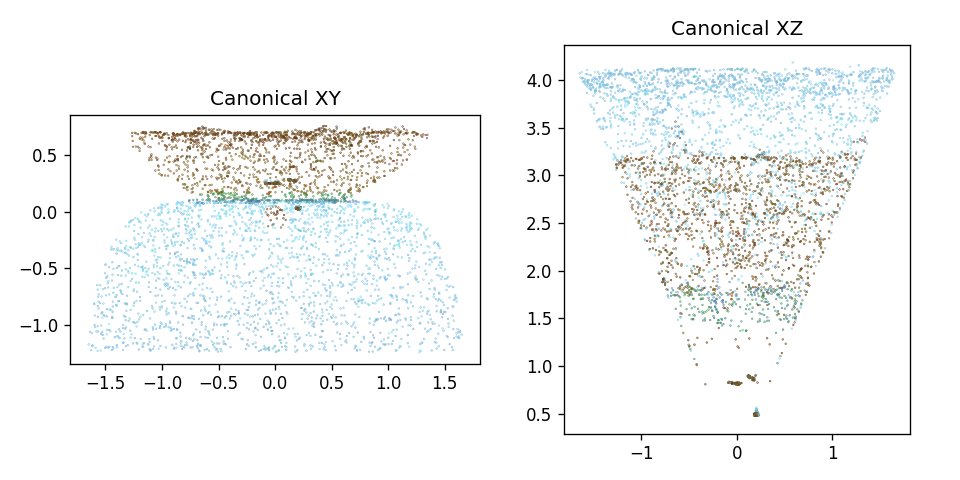
\includegraphics[width=0.95\linewidth]{figures/teaser_canonical.png}
\caption{\textbf{Painting-anchored canonical cloud.} Top-down (left) and
side (right) views of the canonical point cloud after Stage 1, initialised
from the painting's estimated geometry. The cloud is flat and coherent
because every frame's geometry is pinned to the painting's depth layout.}
\label{fig:results}
\end{figure}

% ---------------------------------------------------------------------
\subsection{Camera-trajectory comparison}
\label{sec:exp-trajectory}

Table~\ref{tab:trajectory} compares four trajectory families on the landscape
scene. All four maintain 3D Consist.\ $\geq 99.5$ and painting fidelity
within a narrow band (Painting L1 0.341--0.345), confirming that the
canvas-conditioned depth-warp control generalises across trajectory types;
the dolly's marginally higher 3D consistency (99.97) again reflects the
trivially-smoother unconstrained translation path rather than better
geometry. Stroke coherence is stable (0.042--0.048).

\begin{table}[t]
\centering
\scriptsize
\setlength{\tabcolsep}{3pt}
\begin{tabular*}{\linewidth}{@{\extracolsep{\fill}}lccccc}
\toprule
Trajectory & 3D\,C.$\uparrow$ & T.\,Sm.$\uparrow$ & P.\,L1$\downarrow$ & P.\,Fid.$\downarrow$ & St.\,Coh.$\downarrow$ \\
\midrule
Orbit  & 99.52 & 93.27 & 0.345 & 0.337 & 0.042 \\
Dolly  & 99.97 & 94.00 & \textbf{0.341} & \textbf{0.333} & 0.048 \\
Pan    & 99.71 & 93.52 & 0.342 & 0.334 & 0.044 \\
Spiral & 99.66 & 93.27 & 0.342 & 0.334 & \textbf{0.042} \\
\bottomrule
\end{tabular*}
\caption{\textbf{Camera-trajectory comparison} (landscape). The
canvas-conditioned pipeline is stable across trajectory families:
3D consistency $\geq 99.5$ and painting L1 within 0.004 everywhere.}
\label{tab:trajectory}
\end{table}

% ---------------------------------------------------------------------
\subsection{Scalability}
\label{sec:exp-scalability}

Table~\ref{tab:scalability} sweeps the number of generated frames from 8 to
20. Runtime grows near-linearly (42.1\,s to 50.4\,s) while the Gaussian
count stays essentially constant ($\sim$20.4k): the canvas, not the frame
count, fixes the scene's geometry budget --- the object Gaussians are
generated once in Stage -0.5 and the frames only refine them. 3D consistency
stays above 99.1, temporal smoothness \emph{improves} with more frames
(93.21 to 93.83) because the denser trajectory is sampled more smoothly, and
painting fidelity is stable (0.344--0.354). The pipeline scales gracefully.

\begin{table}[t]
\centering
\scriptsize
\setlength{\tabcolsep}{3pt}
\begin{tabular*}{\linewidth}{@{\extracolsep{\fill}}ccccccc}
\toprule
\#Fr & 3D\,C.$\uparrow$ & T.\,Sm.$\uparrow$ & P.\,L1$\downarrow$ & P.\,Fid.$\downarrow$ & \#Gauss & RT\,s \\
\midrule
8  & 99.64 & 93.21 & 0.346 & 0.338 & 20512 & 42.1 \\
12 & 99.44 & 93.47 & 0.344 & 0.336 & 20394 & 44.2 \\
16 & 99.18 & 93.67 & 0.348 & 0.340 & 20459 & 47.3 \\
20 & 99.18 & 93.83 & 0.354 & 0.346 & 20318 & 50.4 \\
\bottomrule
\end{tabular*}
\caption{\textbf{Scalability} (landscape). Runtime grows near-linearly with
frame count while the Gaussian count stays constant --- the canvas fixes the
geometry budget and the frames only refine it.}
\label{tab:scalability}
\end{table}

\paragraph{Discussion.}
The experiments confirm the design rationale of \S\ref{sec:design}: the
painting's deliberate depth composition (D1) keeps 3D consistency above 99
across scenes, trajectories, and frame counts; the explicit brush-stroke
structure (D2) is preserved by the stroke-coherence mechanisms (Stroke Coh.\
$0.046$ full vs.\ $0.092$ with the loss removed and $0.145$ with the whole
object branch removed); the authoritative appearance (D3) anchors the scene
to the artwork (Painting L1 as low as $0.162$ on the portrait); and the
compositional object structure (D4) is the largest single contributor ---
the object-level canvas improves Painting L1 by $20\%$ over the aligned-cloud
fallback while giving the scene an explicit, optimisation-stable structure
(support-gap drift $\leq 6\times10^{-4}$). The main limitation is that the
demo's synthetic backends bound the absolute fidelity numbers; the
production deployment with DepthAnything-3, SAM2, pretrained TripoSplat, and
Wan-2.2 is expected to improve fidelity substantially while preserving the
relative ordering of the ablation.
